\documentclass[tikz,border=8pt]{standalone}
\usepackage[OT4,plmath]{polski}
\usepackage{amsmath}
\begin{document}
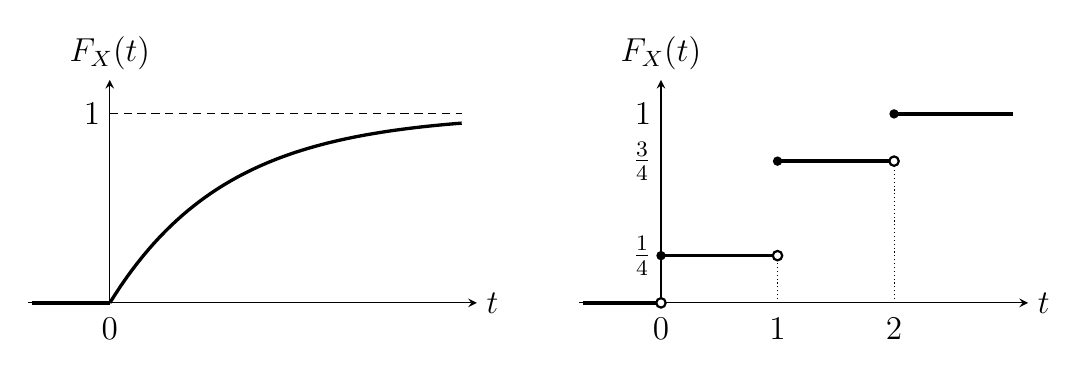
\begin{tikzpicture}[x=1.48cm,y=2.4cm,>=stealth,font=\large]
  \draw[->] (-.7,0)--(3.15,0) node[right] {$t$};
  \draw[->] (0,0)--(0,1.18) node[above] {$F_X(t)$};
  \draw[densely dashed] (0,1)--(3.02,1);
  \node[left] at (0,1) {$1$};
  \node[below] at (0,-.03) {$0$};
  \draw[very thick] (-.67,0)--(0,0);
  \draw[very thick,domain=0:3.02,samples=64] plot (\x,{1-exp(-\x)});
  \begin{scope}[xshift=7cm]
    \draw[->] (-.7,0)--(3.15,0) node[right] {$t$};
    \draw[->] (0,0)--(0,1.18) node[above] {$F_X(t)$};
    \draw[very thick] (-.67,0)--(0,0) (0,.25)--(1,.25)
      (1,.75)--(2,.75) (2,1)--(3.02,1);
    \foreach \x/\lower/\upper in {0/0/.25,1/.25/.75,2/.75/1} {
      \draw[densely dotted] (\x,0)--(\x,\lower);
      \draw[thick,fill=white] (\x,\lower) circle (1.7pt);
      \fill (\x,\upper) circle (1.7pt);
      \node[below] at (\x,-.03) {$\x$};
    }
    \node[left] at (0,.25) {$\frac14$};
    \node[left] at (0,.75) {$\frac34$};
    \node[left] at (0,1) {$1$};
  \end{scope}
\end{tikzpicture}
\end{document}
